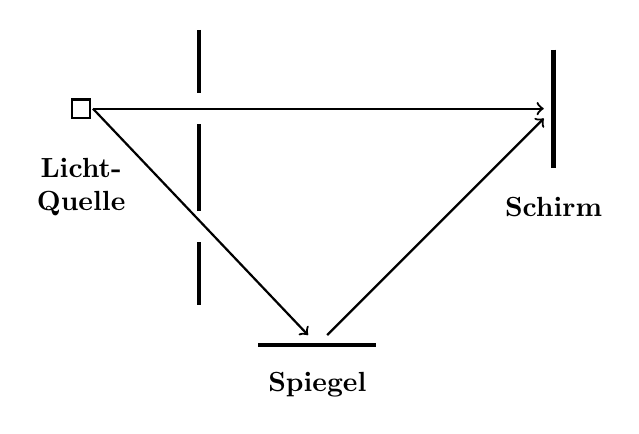
\begin{tikzpicture}
	\node(L)at(-3,0)[rectangle,draw,thick]{};
	\node(P)at(3,0){};
	\node(S)at(0,-3){};

%Beschriftung	
	\node(LQ)at(-3,-1)[align=center]{\textbf{Licht-}\\\textbf{Quelle}};
	\node(Box)at(0,-3.5){\textbf{Spiegel}};
	\node(K)at(3,-1.25){\textbf{Schirm}};
	
	\path [-, ultra thick]
	(-1.5,1)edge(-1.5,0.2)
	(-1.5,-0.2)edge(-1.5,-1.3)
	(-1.5,-1.7)edge(-1.5,-2.5)
	(3,0.75)edge(3,-0.75)         % Schirm
	(-0.75,-3)edge(0.75,-3);      % Spiegel
	
	\path [->, thick]
	(-2.85,0)edge(P)
	(-2.85,0)edge(S)
	(S)edge(P);
\end{tikzpicture}